\documentclass[aspectratio=169]{beamer}

% shared import of packages and command definitions for slides and text

\usepackage{epsfig} % Allows the inclusion of eps files
\usepackage{epic} % Enhanced picture mode
\usepackage{eepic} % Extensions for epic
\usepackage{url} % URL handling
\usepackage{longtable} % Tables that continue onto multiple pages
\usepackage{mathrsfs} % Support for \mathscr script
\usepackage{multirow} % Span rows in tables
\usepackage{bigstrut} % Space struts in tables up and down
\usepackage{amssymb} % AMS math symbols and helpers
\usepackage{graphicx} % Enhanced graphics support
\usepackage{setspace} % Adjust spacing in captions, single by default
\usepackage{xspace} % Automatically adjusting space after macros
\usepackage{amsmath} % \text, and other math formatting options
\usepackage{siunitx} % \num{} formatting and SI unit formatting
\usepackage{booktabs} % Enhanced tables with \toprule, etc.
\usepackage{hyperref} % Add clickable links to other parts of the document
\usepackage{subcaption}
\usepackage{graphicx} % Allows including images

\usepackage[noabbrev,capitalise]{cleveref} % Automatically determine \cref type

% Configure the cleveref package
\newcommand{\creflastconjunction}{, and } % Always use the serial comma

\usepackage[compat=1.1.0]{tikz-feynman} % for feynman diagrams
\tikzfeynmanset{
    warn luatex = {false}
}

\usepackage{hepunits}
% Configure the siunitx package
\sisetup{
    group-separator = {,}, % Use , to separate groups of digits, like 12,345
    list-final-separator = {, and } % Always use the serial comma in \SIlist
}

\newcommand{\fourgev}{\qty{4}{GeV}\xspace}
\newcommand{\eightgev}{\qty{8}{GeV}\xspace}
\newcommand{\ecal}{ECal}
\newcommand{\hcal}{HCal}

\usepackage{acronym}
\acrodef{dm}[DM]{Dark Matter}
\acrodef{sm}[SM]{Standard Model}
\acrodef{gr}[GR]{General Relativity}
\acrodef{cmb}[CMB]{Cosmic Microwave Background}
\acrodef{bao}[BAO]{Baryon Acoustic Oscillations}
\acrodef{hep}[HEP]{High Energy Physics}
\acrodef{wimp}[WIMP]{Weakly Interacting Massive Particle}
\acrodef{ecal}[ECal]{Electromagnetic Calorimeter}
\acrodef{hcal}[HCal]{Hadronic Calorimeter}
\acrodef{ldmx}[LDMX]{Light Dark Matter eXperiment}
\acrodef{hps}[HPS]{Heavy Photon Search experiment}
\acrodef{jlab}[JLab]{Thomas Jefferson National Accelerator Laboratory}
\acrodef{cebaf}[CEBAF]{Continuous Electron Beam Accelerator Facility}
\acrodef{kf}[KF]{Kalman Filter}
\acrodef{gbl}[GBL]{General Broken Lines}
\acrodef{svt}[SVT]{Silicon Vertex Tracker}
\acrodef{bdt}[BDT]{Boosted Decision Tree}
\acrodef{eot}[EoT]{Electrons on Target}
\acrodef{eat}[EaT]{\ac{ecal} as Target}
\acrodef{mm}[MM]{Missing Momentum}
\acrodef{vps}[VPS]{Vertex Projection Significance}

\def\minyzero{$y_{0,\min}$\xspace}
\def\maxyzeroerr{$\sigma_{y_0,\max}$\xspace}

%Environment for drawing on pictures using tikz
%   #1 Width to adjust image to (default: \textwidth)
%   #2 Filepath to image
%Use like:
%   \begin{tikzimage}[height]{filepath}
%       ...\draw...( coordinates are in fractions of width/height of image )
%   \end{tikzimage}
\newenvironment{tikzimage}[2][\textwidth]{%
    \begin{tikzpicture}
        \node[anchor=south west, inner sep=0] (image) at (0,0)
            {\includegraphics[width=#1]{{#2}}};
        \begin{scope}[x={(image.south east)},y={(image.north west)}]
}{%
        \end{scope}
    \end{tikzpicture}
}%


% HPS Diagrams
%   using tikz math library to name variables to helpful names
%   define command to draw boilerplate target/L1/L2
\usetikzlibrary{math}

% colors for diagram
\definecolor{HPSTarget}{rgb}{0.55,0.52,0.54}
\definecolor{HPSTracker}{rgb}{0.0,0.5,0.5}
\definecolor{HPSEcal}{rgb}{0.8,0.5,0.2}

\tikzmath{%
  \openingslope = 0.15; % y changer per x change
  \sensorsep = 0.12; % separation between sensors in a layer
  \sensorlen = 1.5; % length of sensors in vertical direction
  \targetx = -3.0;
  \layeronex = -0.2;
  \layertwox = 2.0;
  \targethalfthick = 0.1;
  \ecalbarlen=1.5;
  \ecalbarwidth=0.3;
  % can't have a blank line in this block
  %
  % compute locations
  \layeroney = (\layeronex - \targetx) * \openingslope;
  \layertwoy = (\layertwox - \targetx) * \openingslope;
  \sensorhalfsep = \sensorsep / 2;
  \reflineendx = \layertwox+0.5;
  \reflineendy = (\reflineendx - \targetx) * \openingslope;
}

\newcommand{\drawhpsfirsttwolayers}{%
  \draw[HPSTracker, very thick]
    (\layeronex-\sensorhalfsep,-\layeroney-\sensorlen)
    -- (\layeronex-\sensorhalfsep,-\layeroney)
    (\layeronex+\sensorhalfsep,-\layeroney-\sensorlen)
    -- (\layeronex+\sensorhalfsep,-\layeroney)
    (\layeronex-\sensorhalfsep,\layeroney+\sensorlen)
    -- (\layeronex-\sensorhalfsep,\layeroney)
    (\layeronex+\sensorhalfsep,\layeroney+\sensorlen)
    -- (\layeronex+\sensorhalfsep,\layeroney);
  \draw[HPSTracker] (\layeronex,\layeroney+\sensorlen) node[above] {L1};
  
  \draw[HPSTracker, very thick]
    (\layertwox-\sensorhalfsep,-\layertwoy-\sensorlen)
    -- (\layertwox-\sensorhalfsep,-\layertwoy)
    (\layertwox+\sensorhalfsep,-\layertwoy-\sensorlen)
    -- (\layertwox+\sensorhalfsep,-\layertwoy)
    (\layertwox-\sensorhalfsep,\layertwoy+\sensorlen)
    -- (\layertwox-\sensorhalfsep,\layertwoy)
    (\layertwox+\sensorhalfsep,\layertwoy+\sensorlen)
    -- (\layertwox+\sensorhalfsep,\layertwoy);
  \draw[HPSTracker] (\layertwox,\layertwoy+\sensorlen) node[above] {L2};
  
  \draw[gray,dashed] (\targetx,0) -- (\reflineendx,\reflineendy);
  \draw[gray,dashed] (\targetx,0) -- (\reflineendx,0);
  \draw[gray,dashed] (\targetx,0) -- (\reflineendx,-\reflineendy);
  
  \fill[HPSTarget] (\targetx-\targethalfthick,+1) rectangle (\targetx+\targethalfthick,-1);
  \draw[HPSTarget] (\targetx,-1) node[below] {Target};
}

\newcommand{\drawhps}{%
  \foreach \layerX/\layerY in {
    0.0/0.15,
    2.0/0.30,
    4.0/0.45,
    6.0/0.60,
    8.0/0.75,
    10.0/0.90
  }{
    \draw[HPSTracker, very thick]
      (\layerX-\sensorhalfsep,-\layerY-\sensorlen)
      -- (\layerX-\sensorhalfsep,-\layerY)
      (\layerX+\sensorhalfsep,-\layerY-\sensorlen)
      -- (\layerX+\sensorhalfsep,-\layerY)
      (\layerX-\sensorhalfsep,\layerY+\sensorlen)
      -- (\layerX-\sensorhalfsep,\layerY)
      (\layerX+\sensorhalfsep,\layerY+\sensorlen)
      -- (\layerX+\sensorhalfsep,\layerY);
  }
  \draw[HPSTracker] (9.0,0.75+\sensorlen) node[above,font=\LARGE] {SVT};

  \foreach \barY in {
    0.9,
    1.2,
    1.5,
    1.8,
    2.1
  }{
    \draw[draw=HPSEcal,fill=HPSEcal!20!white]
      (12.0,\barY) rectangle (12+\ecalbarlen,\barY+\ecalbarwidth)
      (12.0,-\barY) rectangle (12+\ecalbarlen,-\barY-\ecalbarwidth)
    ;
  }
  \draw[HPSEcal] (12+\ecalbarlen/2,2.1+\ecalbarwidth) node[above,font=\LARGE] {ECal};

  \draw[gray,dashed] (\targetx,0) -- (12+\ecalbarlen+0.5,0);
  
  \fill[HPSTarget] (\targetx-\targethalfthick,+1) rectangle (\targetx+\targethalfthick,-1);
  \draw[HPSTarget] (\targetx,-1) node[below left,font=\LARGE] {Target};

  \node (decay) at (\targetx+1.0,0.05) [circle,fill,inner sep=1.5pt] {};
  \node (production) at (\targetx,0.0) [circle,fill,inner sep=1.5pt] {};

  \draw[black,very thick,->]
    (\targetx-1.5,0.0) node[anchor=south east,font=\Large] {\(e^-\)} -- (\targetx-0.2,0.0);
  \draw[black,very thick,->]
    (decay) -- (11.8,1.6) node[anchor=south east,font=\Large] {\(e^-\)};
  \draw[black,very thick,->]
    (decay) -- (11.8,-2.2) node[anchor=north east,font=\Large] {\(e^+\)};
  \draw[black,very thick,->]
    (production) -- (-1.0,-0.5-\sensorlen) node[anchor=east,font=\Large] {\(e^-\)};

  \draw[blue,thick,->] (production) -- (decay) node[midway,above,font=\Large] {\(V_D\)};
}


\mode<presentation> {
  \usetheme{Madrid}

  \addtobeamertemplate{frametitle}{}{
      \begin{textblock*}{100mm}(0.8\textwidth,-0.95cm)
          
\includegraphics[height=0.95cm]{ldmx_logo}
      \end{textblock*}
      \begin{textblock*}{100mm}(0.7\textwidth,-0.95cm)
        
\includegraphics[height=0.95cm]{heavy_photon_logo}
      \end{textblock*}
  }

  \setbeamercolor{structure}{fg = UMNStormy }

  \setbeamercolor{palette primary}{fg = UMNMaroon, bg = UMNLightGray}
  \setbeamercolor{palette secondary}{fg = UMNMaroon, bg = white }
  \setbeamercolor{palette tertiary}{fg = UMNLightGold, bg = UMNStormy}

  \setbeamercolor{frametitle}{fg = UMNLightGold, bg = UMNMaroon }
  \setbeamercolor{title}{fg = UMNMaroon, bg = UMNLightGray }

  \setbeamercolor{section in toc}{fg = UMNMaroon}
  \setbeamercolor{section in toc shaded}{fg = UMNMaroon}
  
  \setbeamercolor{button}{fg = UMNLightGold, bg = UMNMaroon }
  
  \setbeamercolor{palette sidebar secondary}{fg = UMNMaroon }
  \setbeamercolor{section in sidebar shaded}{fg = UMNMaroon }

  \setbeamertemplate{itemize item}{\color{UMNMaroon}$\blacksquare$}
  \setbeamertemplate{itemize subitem}{\color{UMNLightGold}$\blacktriangleright$}
  \setbeamertemplate{enumerate items}[default]
  \setbeamertemplate{sections/subsections in toc}[sections numbered]

  \setbeamertemplate{navigation symbols}{} % To remove the navigation symbols from the bottom of all slides

  \setbeamercolor{block body alerted}{fg = UMNSunny, bg = UMNMaroon!20}
  \setbeamercolor{block title alerted}{fg = UMNLightGold, bg = UMNMaroon}
}

\def\with{}

\author{Tom Eichlersmith} % Your name
\institute[UMN] % Your institution as it will appear on the bottom of every slide, may be shorthand to save space
{
he/him/his \\ \medskip
University of Minnesota \\ \medskip
\href{mailto:eichl008@umn.edu}{eichl008@umn.edu} \\ \medskip
\begin{tabular}{p{0.4\textwidth}} \centering\with \end{tabular}
}





\usepackage{pgfpages}
\setbeamertemplate{note page}[plain]
\setbeameroption{show notes}
%\setbeameroption{show notes on second screen}

\newcommand{\ssection}[1]{%
  \section{#1}%
  \sectionframe{#1}%
}%

\newenvironment{sframe}[1]{%
  \subsection{#1}%
  \begin{frame}{#1}%
}{%
  \end{frame}%
}%

\title[Fixed Target DM Searches: HPS and LDMX]{%
  Searches for Dark Matter Production in Two Fixed Target Experiments: HPS and LDMX%
}

\begin{document}

\begin{frame}
  \maketitle
\end{frame}

\note[itemize]{
\item Welcome, I'll be talking about my disseration research focused
  on two fixed target experiments (HPS and LDMX) looking for the production
  of dark matter.
\item Please offer feedback -- first attempt to unify the two experiments into one talk.
\item Trying to focus on making talk cohesive
}

\begin{frame}{Outline}
  \begin{columns}
    \begin{column}{0.5\textwidth}
      \tableofcontents
    \end{column}
    \begin{column}{0.5\textwidth}
      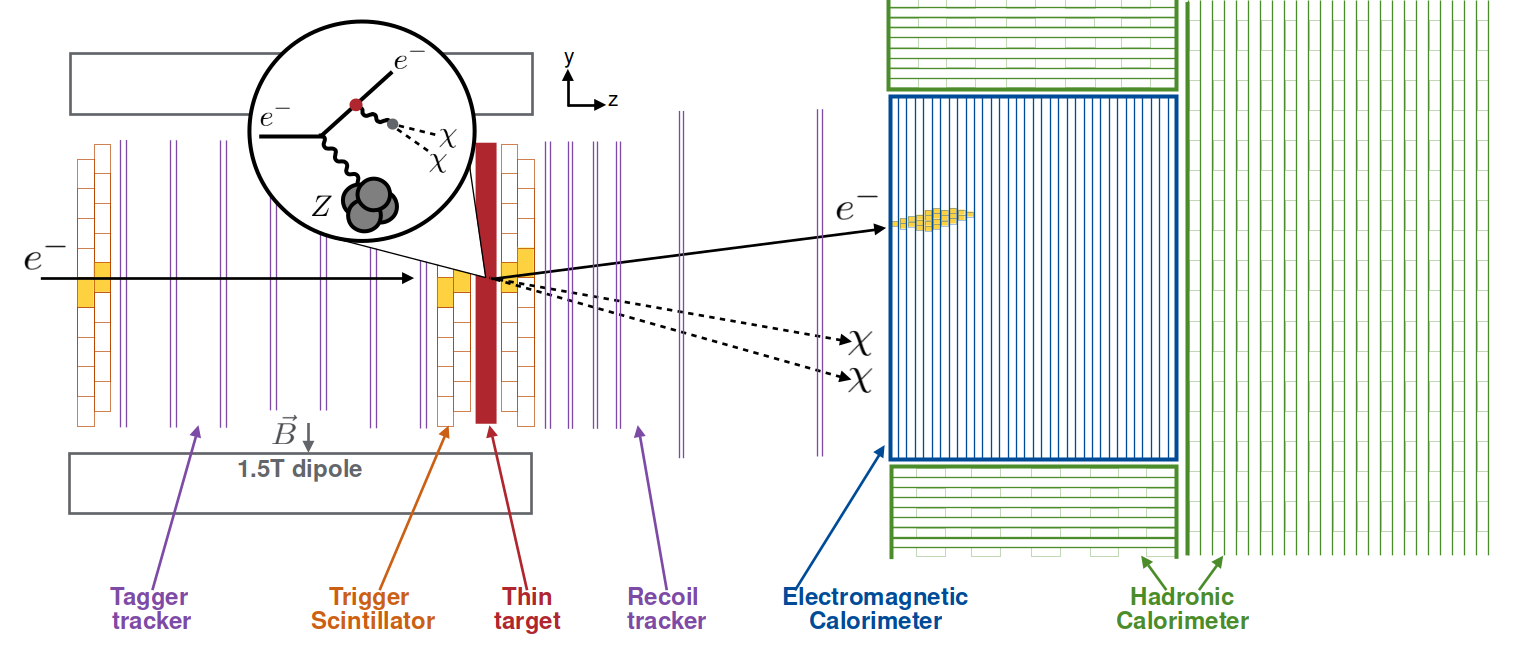
\includegraphics[width=\textwidth]{../figures/ldmx/experiment/detector.png}
      \\
      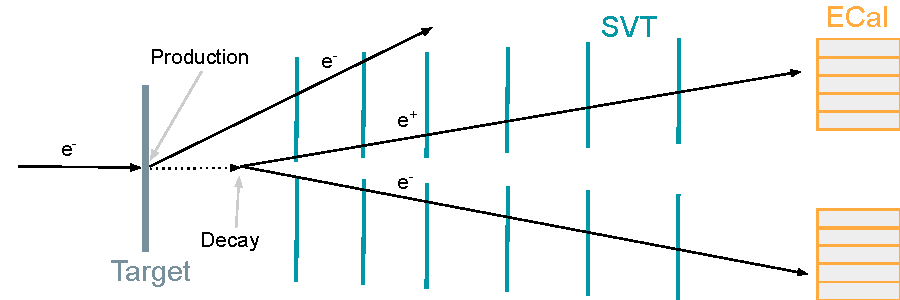
\includegraphics[width=\textwidth]{../figures/hps/experiment/hps-diagram.pdf}
    \end{column}
  \end{columns}
\end{frame}

\note[itemize]{
\item Background to get us on the same footing and using the same vocabulary
\item Motivate category of DM that experiments are searching for
\item Go through my analyses within both experiments
}

\ssection{Background}

\subsection{HEP Vocabulary}

\begin{frame}{Standard Model}
  \begin{columns}
    \begin{column}{0.4\textwidth}
      \begin{figure}
        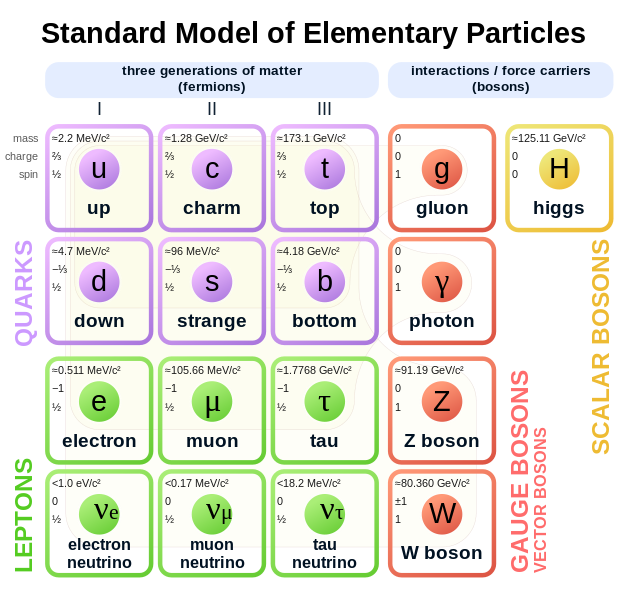
\includegraphics[width=\textwidth]{../figures/intro/Standard_Model_of_Elementary_Particles.svg.png}
        \caption{Credit to user Cush on wikipedia for providing this diagram.}
      \end{figure}
    \end{column}
    \begin{column}{0.6\textwidth}
      \begin{itemize}
        \item \boldcol{UMNSunny}{Law} -- summary of a set of consistent observations about phenomena
        \item \boldcol{UMNSunny}{Model} -- package of ``laws'' and their mathematical forms from which we can make predictions about future observations
        \item \boldcol{UMNSunny}{Orthogonal} -- used to emphasize that two different analyses are statistically independent
      \end{itemize}
    \end{column}
  \end{columns}
\end{frame}

\note[itemize]{
\item Laws are summaries of observations and models
  are just packaging these laws with some mathematical sugar
\item The SM is the most quantitatively accurate physics model ever known to human kind.
\item It is a package of particles and their interactions (also represented by particles)
  from which we can -- with a specific mathematical framework -- make predictions about
  our observations.
\item \textbf{BUT} it fails to account for all observed phenomena (e.g. \emph{gravity})
}

%\begin{frame}{Feynman Diagram}
%\end{frame}
%
%\begin{frame}{Particle Mixing}
%  \begin{columns}
%    \begin{column}{0.4\textwidth}
%      \begin{figure}
%        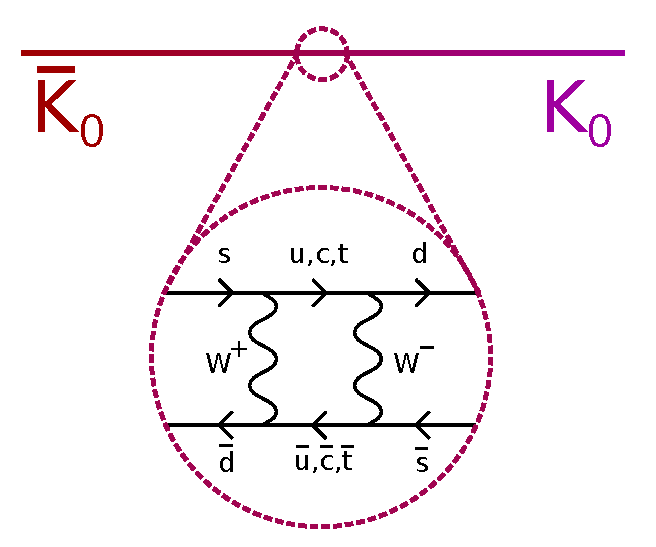
\includegraphics[width=\textwidth]{%
%          ../figures/intro/Kaon-box-diagram-with-bar.pdf%
%        }
%        \caption{Figure created by user NikNaks on Wikipedia.}
%      \end{figure}
%    \end{column}
%  \end{columns}
%\end{frame}
%
%\begin{frame}{Displaced Decay Vertices}
%  \begin{columns}
%    \begin{column}{0.5\textwidth}
%      \begin{figure}
%        \begin{tikzimage}[0.6\textwidth]{../figures/intro/bubble-chamber.jpeg}
%          \definecolor{brilliantrose}{rgb}{1.0, 0.33, 0.64}
%          % \draw[step=0.1,black,thin] (0.0,0.0) grid (1.0,1.0);
%          \node (prod) at (0.4,0.54) {};
%          \node[circle,draw=brilliantrose] (decay) at (0.515,0.54) {};
%          \draw[dashed,brilliantrose,thick] (prod) -- (decay);
%      
%          \node (beam1) at (0.1,0.5) {\color{brilliantrose}\(\pi^-\)};
%          \node (beam2) at (0.2,0.5) {};
%          \draw[->,brilliantrose,thick] (beam1) -- (beam2);
%        \end{tikzimage}
%        \caption{Image of CERN's first liquid hydrogen bubble chamber from 1960.}
%      \end{figure}
%    \end{column}
%  \end{columns}
%\end{frame}

\subsection{Dark Matter}
\begin{frame}{Dark Matter}
  \begin{columns}
    \begin{column}{0.5\textwidth}
      \begin{figure}
        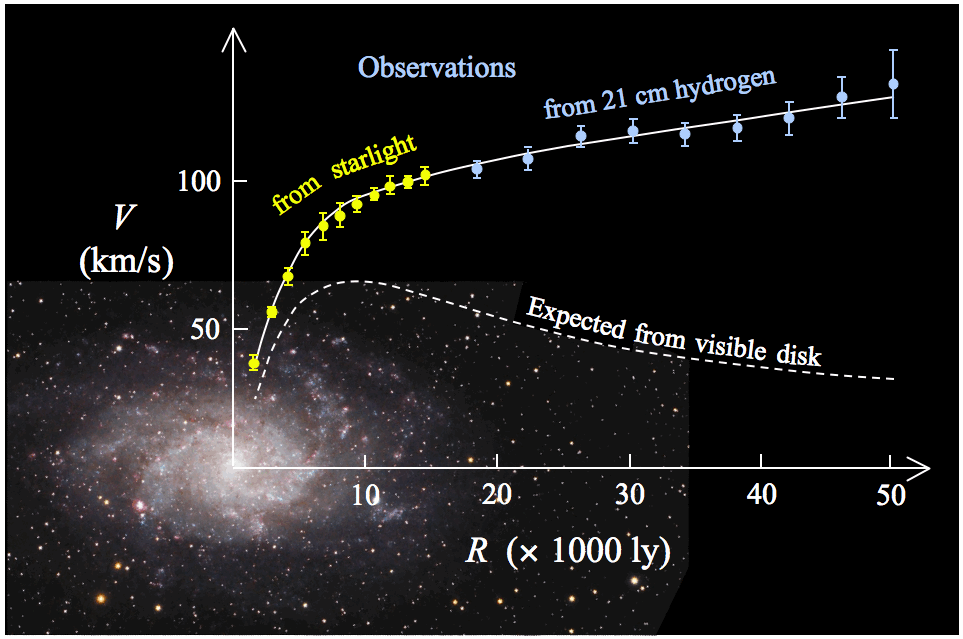
\includegraphics[width=\textwidth]{../figures/theory/rotation-curve-evidence-for-dm.png}
        \caption{Stuff is spinning too fast!}
      \end{figure}
    \end{column}
    \begin{column}{0.5\textwidth}
      \begin{figure}
        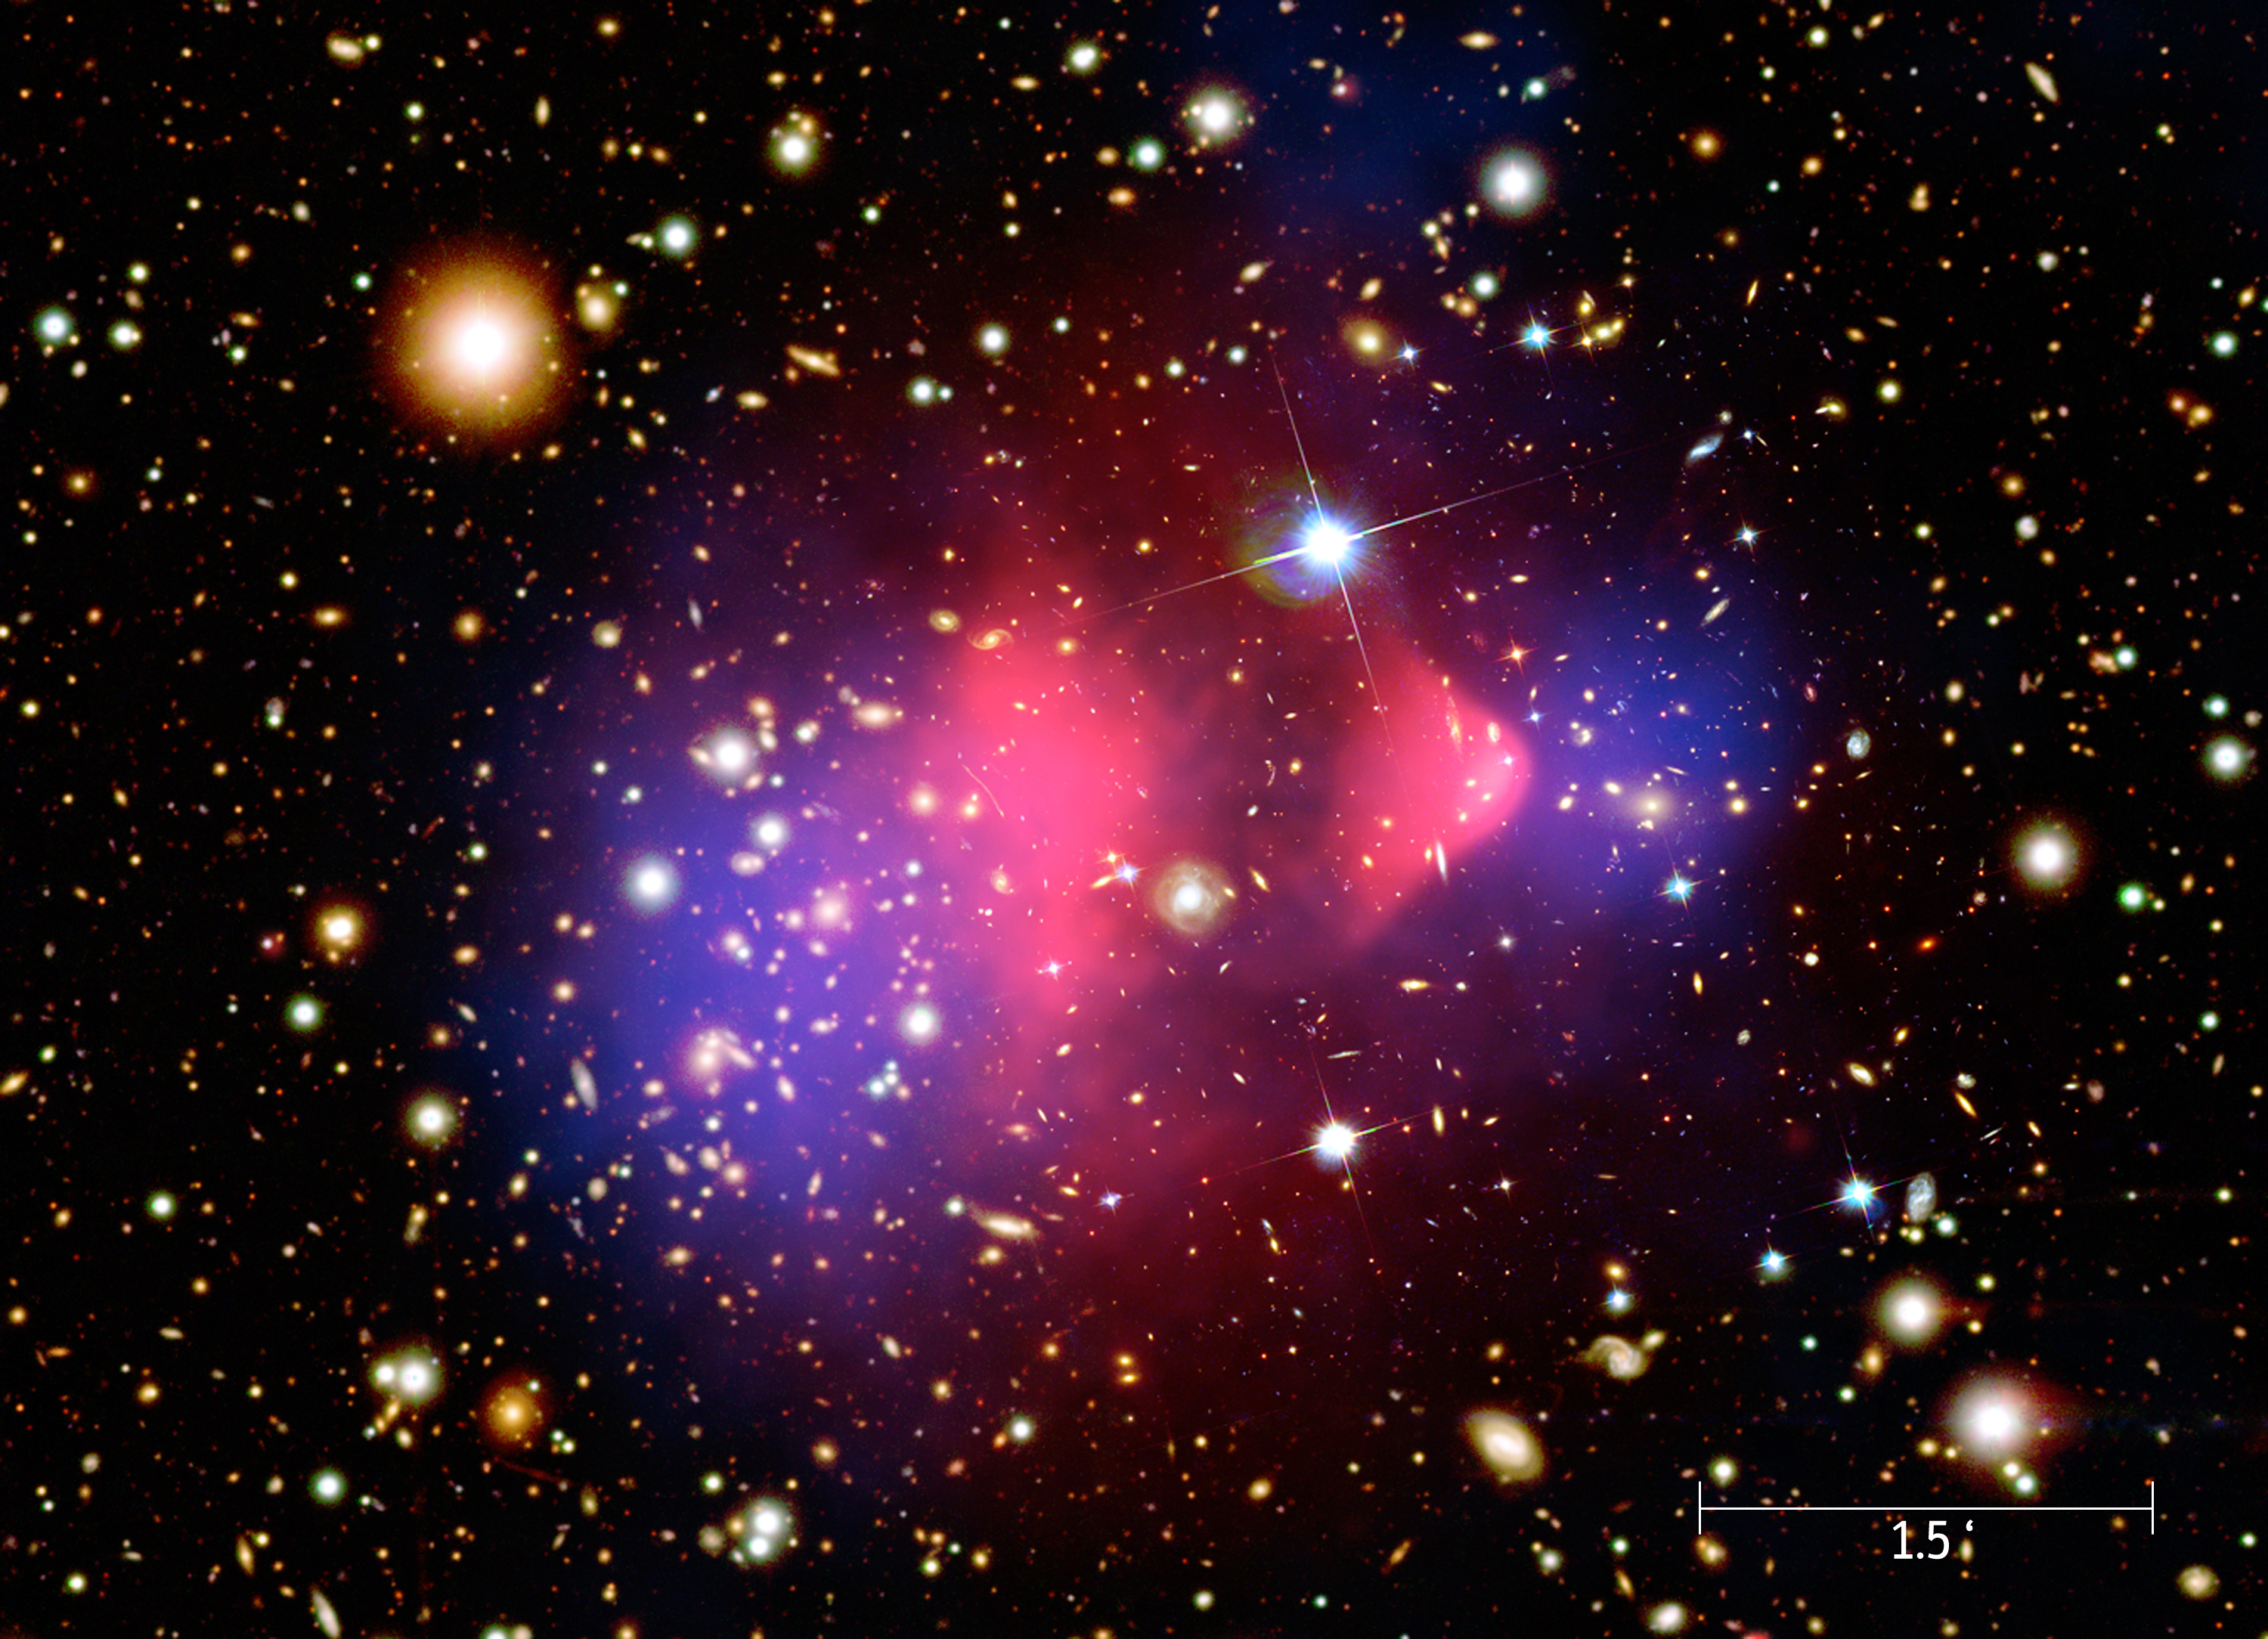
\includegraphics[width=\textwidth]{%
          ../figures/intro/bullet-cluster.jpg
        }
        \caption{Gravitational lensing (blue) and infrared (pink) observations
        show mass in different places!}
      \end{figure}
    \end{column}
  \end{columns}
\end{frame}

\note[itemize]{
\item One of the phenomena the SM doesn't account for is DM
\item We know it exists
}

\begin{frame}{Thermal Relic Dark Matter}
  \begin{block}{Narrow Wealth of Possibilities}
    Make the simple assumption that \ac{dm} has always been here.
  \end{block}
  \vfill
  \begin{figure}
    \centering
    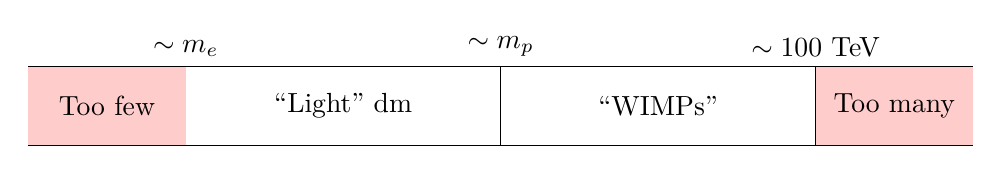
\begin{tikzpicture}
    % horizontal top/bottom lines
    \draw (0,0) -- (12,0);
    \draw (0,1) -- (12,1);
    % dividing lines along with relevant scale markers
    \draw (2,0) -- (2,1) node[above] {$\sim m_e$};
    \draw (6,0) -- (6,1) node[above] {$\sim m_p$};
    \draw (10,0) -- (10,1) node[above] {$\sim100~$TeV};
    % fill non-thermal ranges with light red
    \fill [red!20!white] (0,0) rectangle (2,1);
    \fill [red!20!white] (10,0) rectangle (12,1);
    % labels offering descriptions of ranges inside the boxes
    \node at (1,0.5) {Too few};
    \node at (4,0.5) {``Light'' \gls{dm}};
    \node at (8,0.5) {``WIMPs''};
    \node at (11,0.5) {Too many};
\end{tikzpicture}
    \caption{Mass scale of Thermal Relic \ac{dm}.
      The regions in red are excluded by applying the thermal relic assumption
      to our observations of the universe's early evolution.}
    \label{fig:dm-mass-scale}
  \end{figure}
  \boldcol{UMNSunny}{Both LDMX and HPS are searching for production of Light DM with electrons.}
\end{frame}

\note[itemize]{
\item Simplifying assumption: Dark Matter has always been here (like standard matter)
  and was in thermal equilibrium with standard matter in the early universe
\item (Observations of the CMB also imply this so its a decently motivated assumption.)
\item Limits the scale of mass of DM particles by connecting the mass to the interaction
  strength
\item Above $m_p\sim\qty{1}{\GeV}$, the interaction could be provided by the standard Weak
  force (so-called WIMPs), many experiments searching in this region
\item Below $m_p$, the interaction needs to be even weaker than the standard Weak force
\item Particles are lighter than WIMPs so referred to as Light DM
}

\begin{frame}{A Benchmark Model}
  \begin{columns}
    \begin{column}{0.5\textwidth}
      \begin{figure}
        \centering
        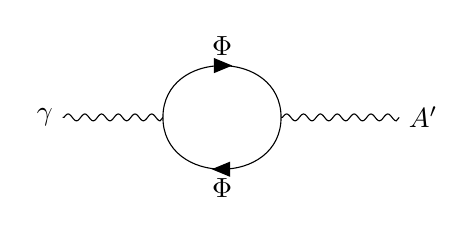
\begin{tikzpicture}
  \begin{feynman}
    \vertex (standard) {\(\gamma\)};
    \vertex [right=of standard] (loopleft);
    \vertex [right=of loopleft] (loopright);
    \vertex [right=of loopright] (dark) {\(A'\)};

    \diagram*{
    (standard)
    -- [photon] (loopleft)
    -- [fermion, half left, edge label=\(\Phi\)] (loopright)
    -- [photon] (dark),
    (loopright)
    -- [fermion, half left, edge label=\(\Phi\)] (loopleft),
    };
  \end{feynman}
\end{tikzpicture}

        \caption{Heavy field $\Phi$ enabling mixing between standard and dark photons.}
      \end{figure}

      The required connection between standard and dark sector provides an
      effective mixing of the standard and dark photons at our energy scales.
    \end{column}
    \begin{column}{0.5\textwidth}
      \begin{figure}
        \centering
        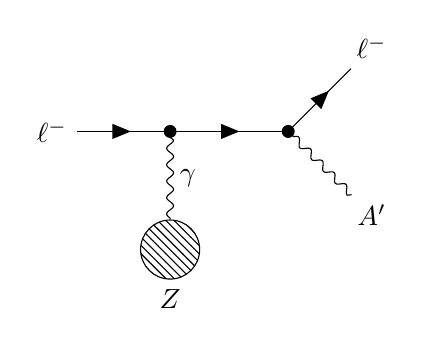
\begin{tikzpicture}
  \begin{feynman}
    \vertex (in) {\(\ell^-\)};
    \vertex [right=of in, dot] (nuc) {};
    \vertex [below=of nuc, blob, label={below:\(Z\)}] (nucleus) {};
    \vertex [right=of nuc, dot] (emit) {};
    \vertex [above right=of emit] (recoil) {\(\ell^-\)};
    \vertex [below right=of emit] (decay) {\(A'\)};
    % \vertex [above right=of decay] (chi2) {\(\overline{\chi}\)};
    % \vertex [below right=of decay] (chi1) {\(\chi\)};

    \diagram*{
    (in) -- [fermion] (nuc) -- [fermion] (emit) -- [fermion] (recoil),
    (nucleus) -- [photon, edge label'=\(\gamma\)] (nuc),
    (emit) -- [photon] (decay),
    % (emit) -- [photon, edge label'=\(A'\)] (decay),
    % (chi2) -- [fermion] (decay) -- [fermion] (chi1),
    };
  \end{feynman}
\end{tikzpicture}

        \caption{Dark bremsstrahlung process.}
      \end{figure}
      
      Mixing allows for a new process producing dark particles

      \boldcol{UMNSunny}{Both HPS and LDMX search for this production mechanism}
    \end{column}
  \end{columns}
\end{frame}

\note[itemize]{
\item The thermal relic assumption combined with curiosity for the lower masses
  requires the introduction of a new field which is presumably much heavier
  (i.e. harder to produce and observe) than our current energies.
\item This required connection does provide an effictive mixing of the standard
  and dark photons (like how kaons can mix) at our energy scales
\item Allowing for this mixing then gives a new process that can produce
  dark particles in our experiments -- dark bremsstrahlung
\item Both HPS and LDMX search for dark brem; however, they have different
  tactics to look for it
}

\ssection{LDMX}

\note[itemize]{
\item First, let's talk about the experiment I started with
\item The Light Dark Matter eXperiment is a \textbf{Missing Momentum} search for
  the dark bremsstralung production of dark particles with an electron beam
\item i.e. We assume that the dark photon that is produced ``stays in'' the dark sector
  and the momentum it had is not observable by our detector
}

\subsection{Experiment}
\begin{frame}{Missing Momentum Search}
  \begin{columns}
    \begin{column}{0.25\textwidth}
      \begin{block}{To Do MM Search}
        Need faithful ID of even very rare SM processes
      \end{block}
    \end{column}
    \begin{column}{0.7\textwidth}
      \begin{figure}
        \centering
        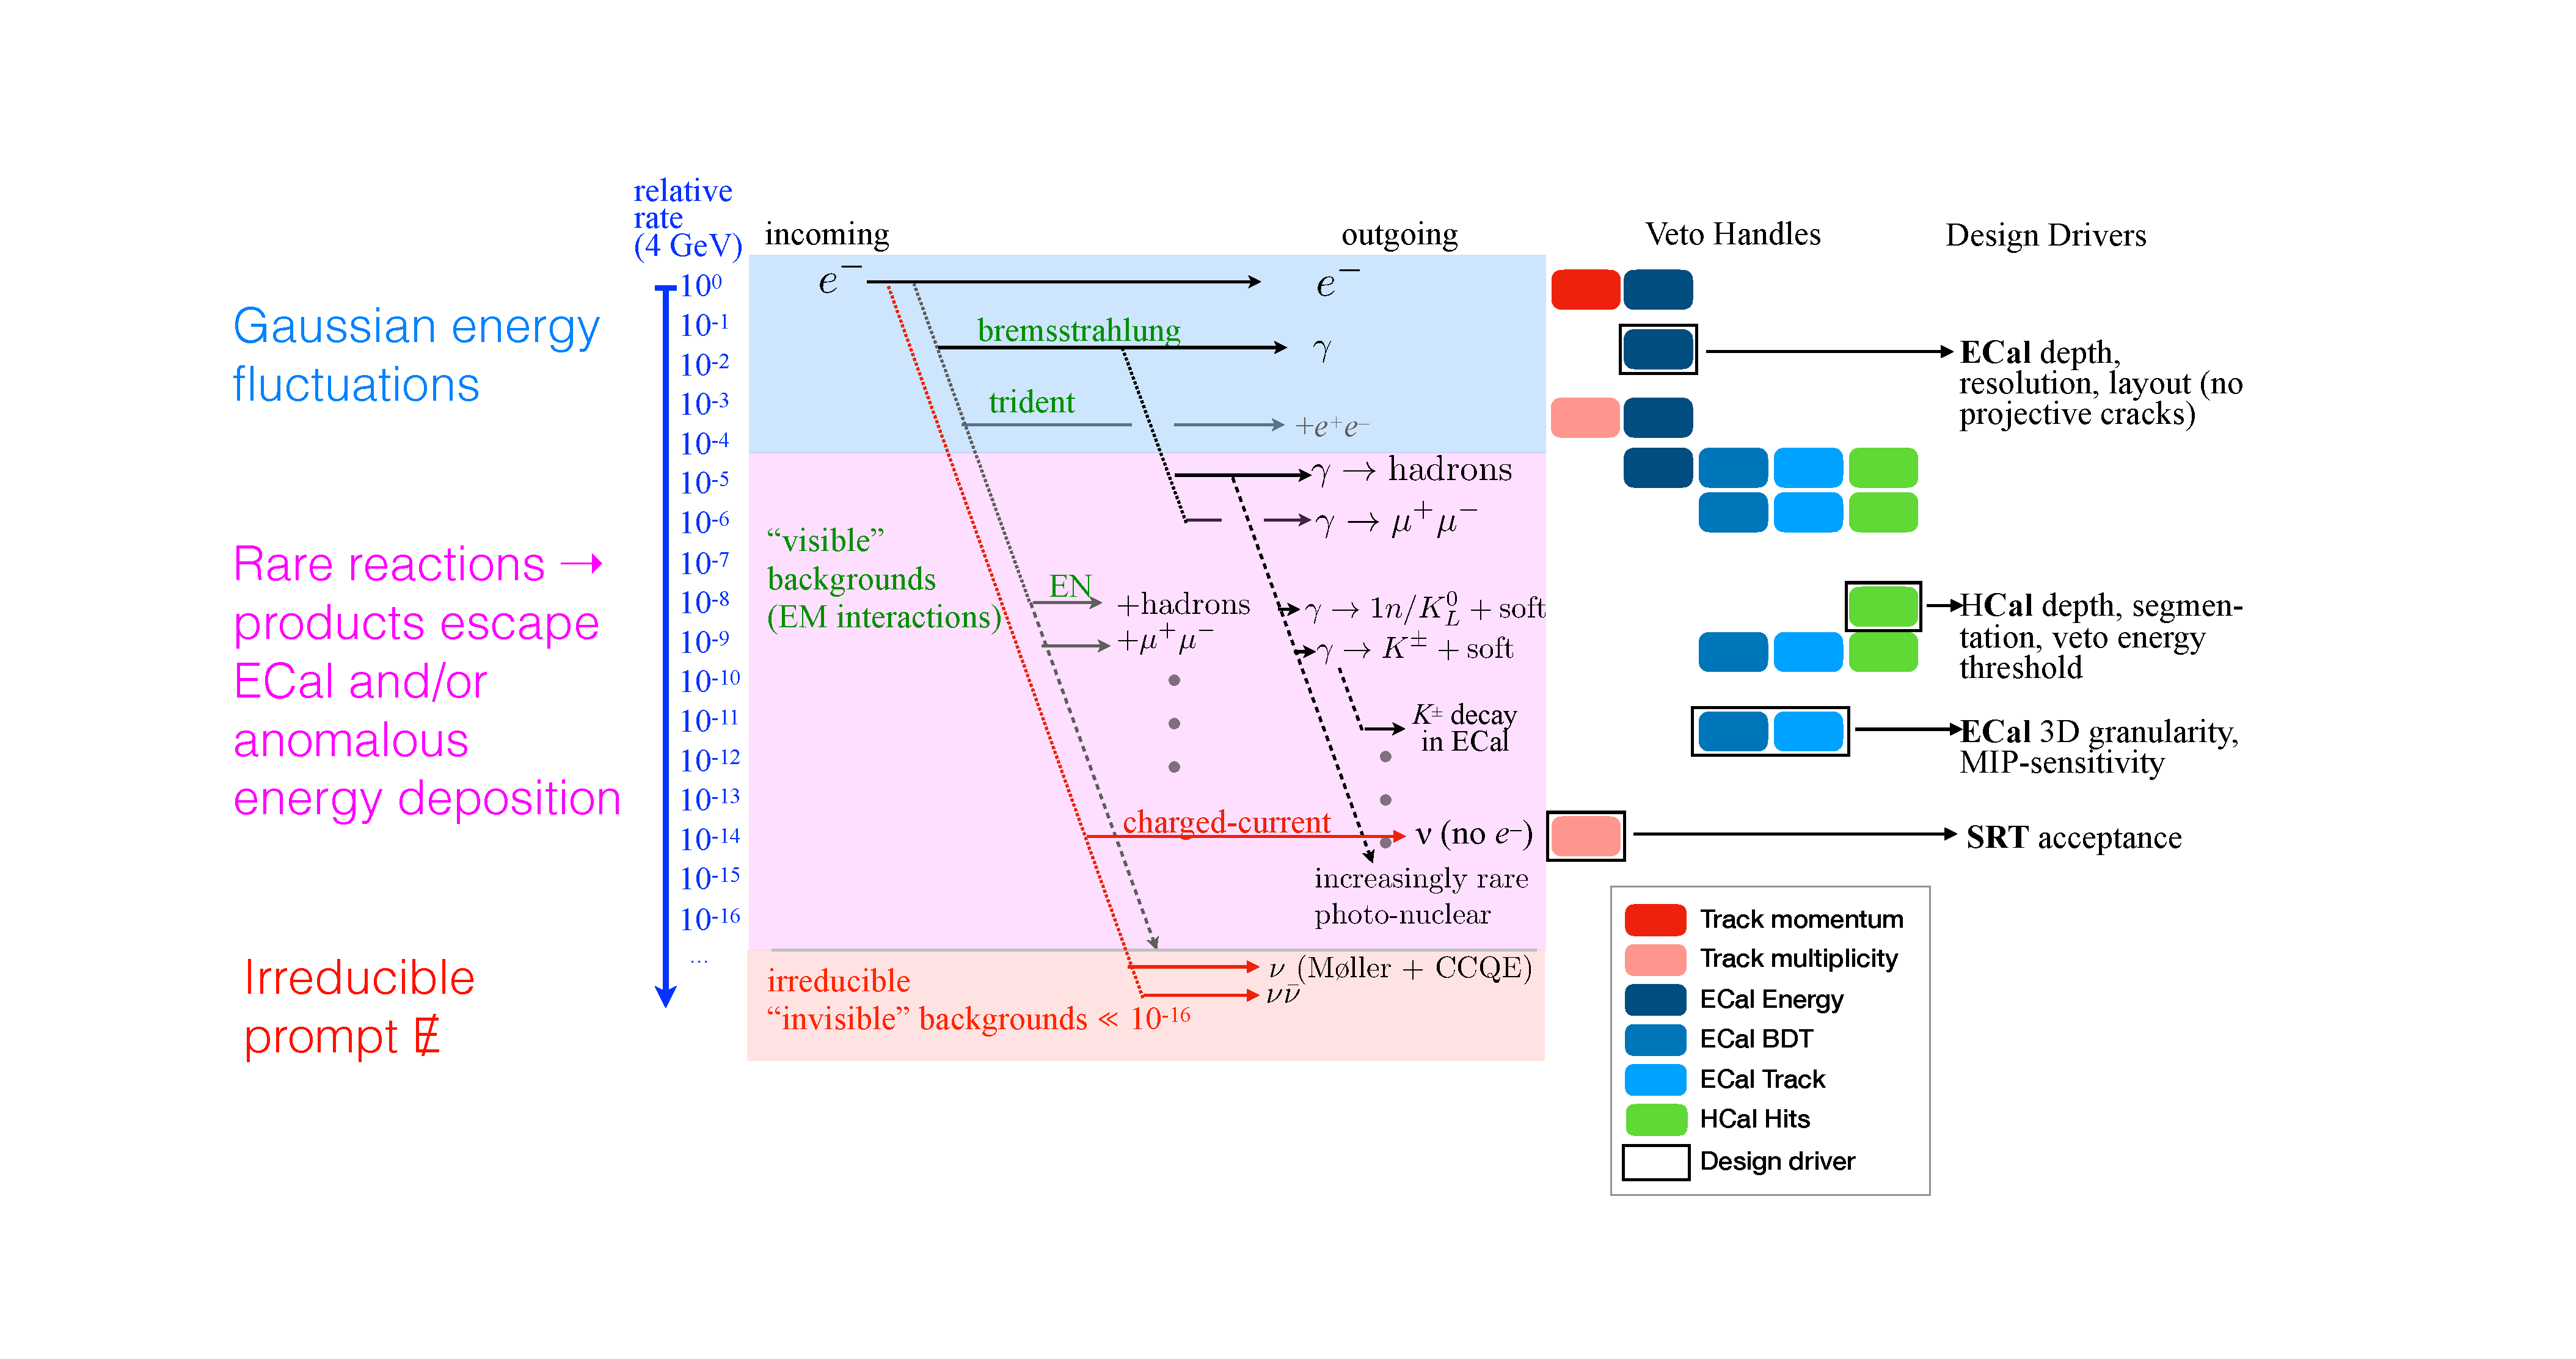
\includegraphics[width=\textwidth]{../figures/ldmx/experiment/reaction_staircase_with_designDrivers.pdf}
        \caption{Credit to Tim Nelson}
      \end{figure}
    \end{column}
  \end{columns}
\end{frame}

\note[itemize]{
\item LDMX, as mentioned, is a MM search and, to do MM, we need to be able to faithfully
  ID very rare SM processes
\item Here is a diagram of prominent SM processes ordered by their relative rate
\item Blue -- high rate processes that we can ID with fast total energy calculation 
  (given we know how many electrons are coming in)
\item Pink -- rarer processes that are more complicated requiring more granular
  information about what happens to the products of the electron's interactions
  (hadronic calorimeter, silicon recoil tracker)
\item Red -- very rare processes that we will not be able to remove
  (but could constrain using measurements of these processes by other experiments)
}

\begin{frame}{Experiment}
  \begin{figure}
    \centering
    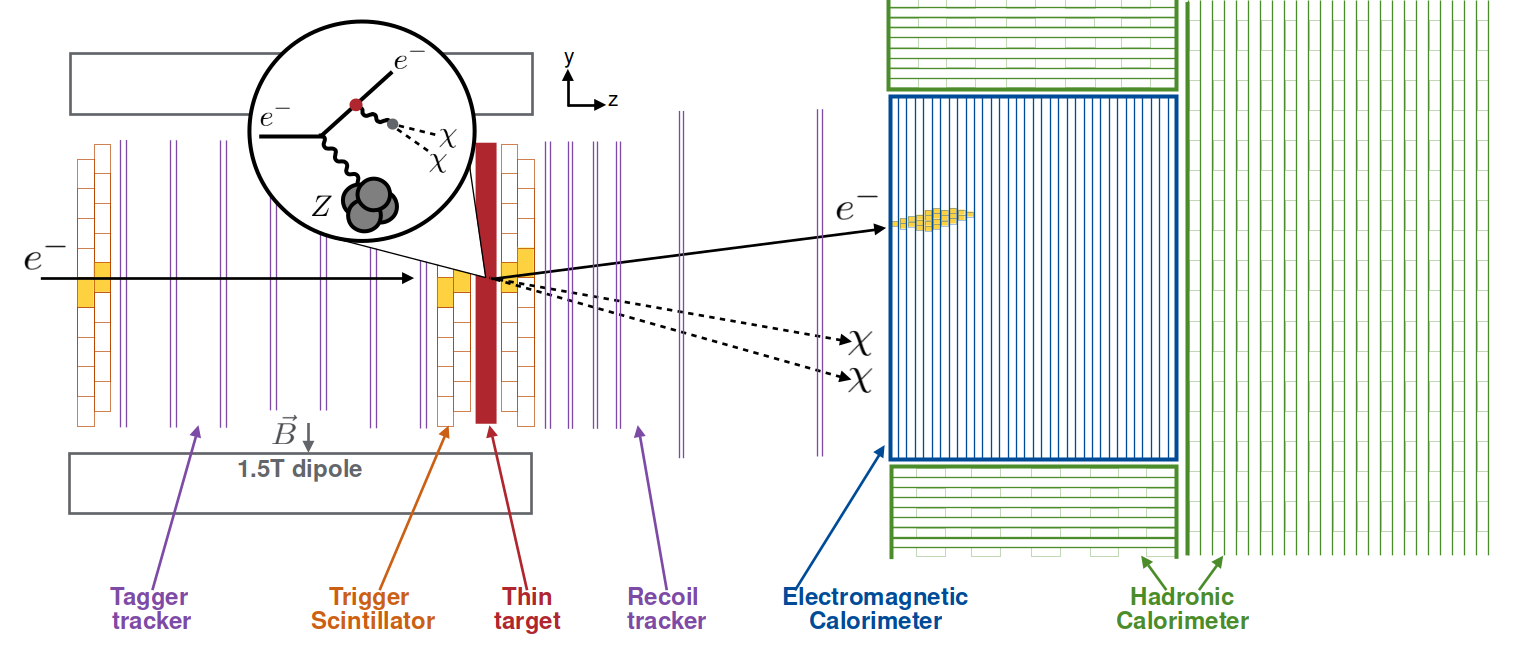
\includegraphics[width=\textwidth]{../figures/ldmx/experiment/detector.png}
    \caption{Credit to Christian Herwig for original diagram}
  \end{figure}
\end{frame}

\note[itemize]{
\item These processes motivate a staged design
  \begin{itemize}
    \item a tracker (tagger for incoming and recoil for outgoing)
    \item ECal for electrons/positrons and photons
    \item HCal for hadrons (e.g. protons/neutrons) and muons
    \item a TrigScint to quickly count electrons and help ECal make trigger decision in time.
  \end{itemize}
\item Hosted at SLAC Natl Accelerator Lab, recieving beam from LCLS-II 
\item Beam facility upgrading from \qty{4}{\GeV} to \qty{8}{\GeV}, LDMX may see
  some \qty{4}{\GeV} beam depending on how schedules line up but a majority
  of data will be taken with \qty{8}{\GeV}
\item \textbf{Thin target to help momentum resolution.} -- most electrons pass through
  only minimally interacting
\item Can we still use this data we would collect anyways?
}

\subsection{New, Orthogonal Analysis Channel}
\begin{frame}{Using the ECal as Target}
  \begin{figure}
    \centering
    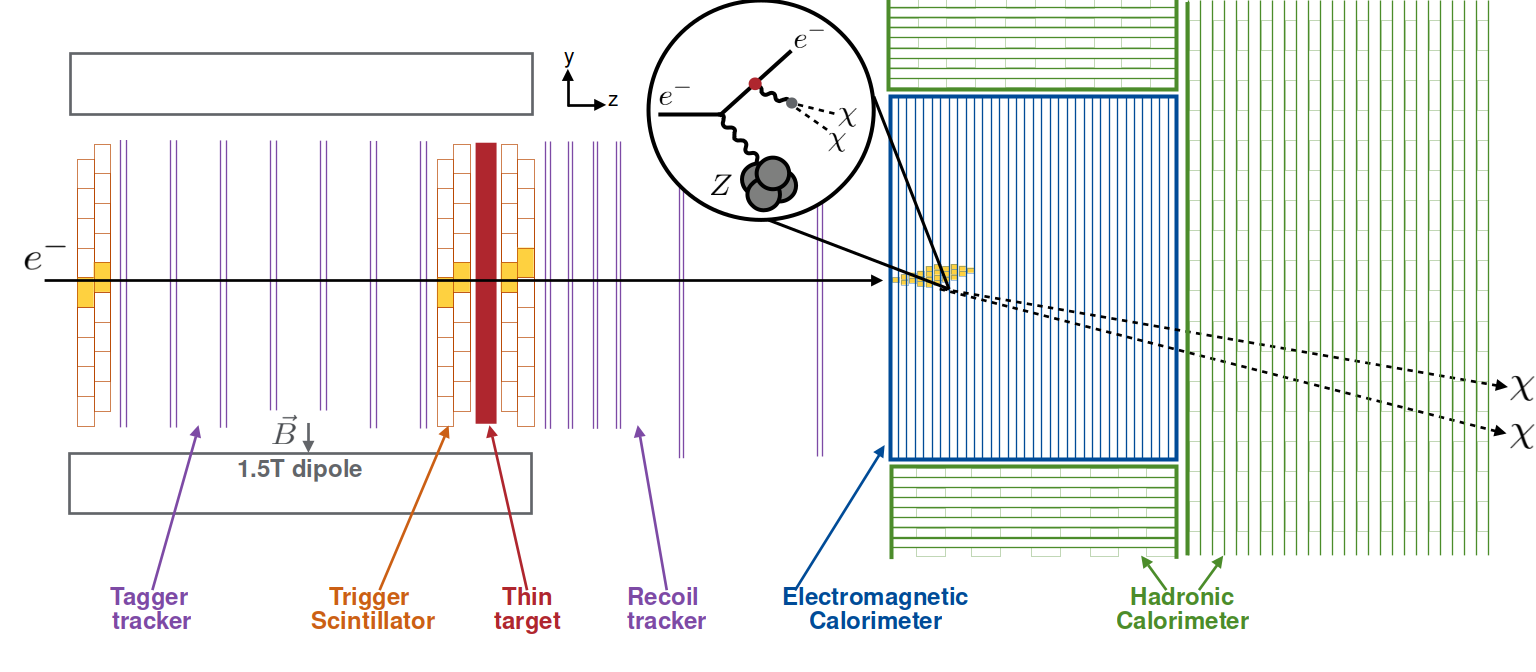
\includegraphics[width=\textwidth]{figs/detector-eat-signal.png}
    \caption{Credit to Christian Herwig for original diagram}
  \end{figure}
\end{frame}

\note[itemize]{
\item Yes we can!
\item If the dark brem process exists and would happen in the thin target,
  it would also happen within other parts of our detector -- namely the ECal
  which has a lot of material and would recieve similar numbers of electrons as
  the target
\item Use the Ecal as another Target for our dark brem search
\item Shift focus to \textbf{Missing Energy} search
\item Use upstream detectors to confirm near-beam-energy electron entering ECal \\
  (orthogonality condition, MM search requires significant loss within thin target)
\item ECal has more material $\to$ more ``chances'' for dark brem to happen \\
  (about $\sim 3$ times more when accounting for acceptance and trigger efficiency)
}

\begin{frame}{Familiar Culprits}
  \begin{columns}
    \begin{column}{0.45\textwidth}
      \begin{figure}
        \centering
        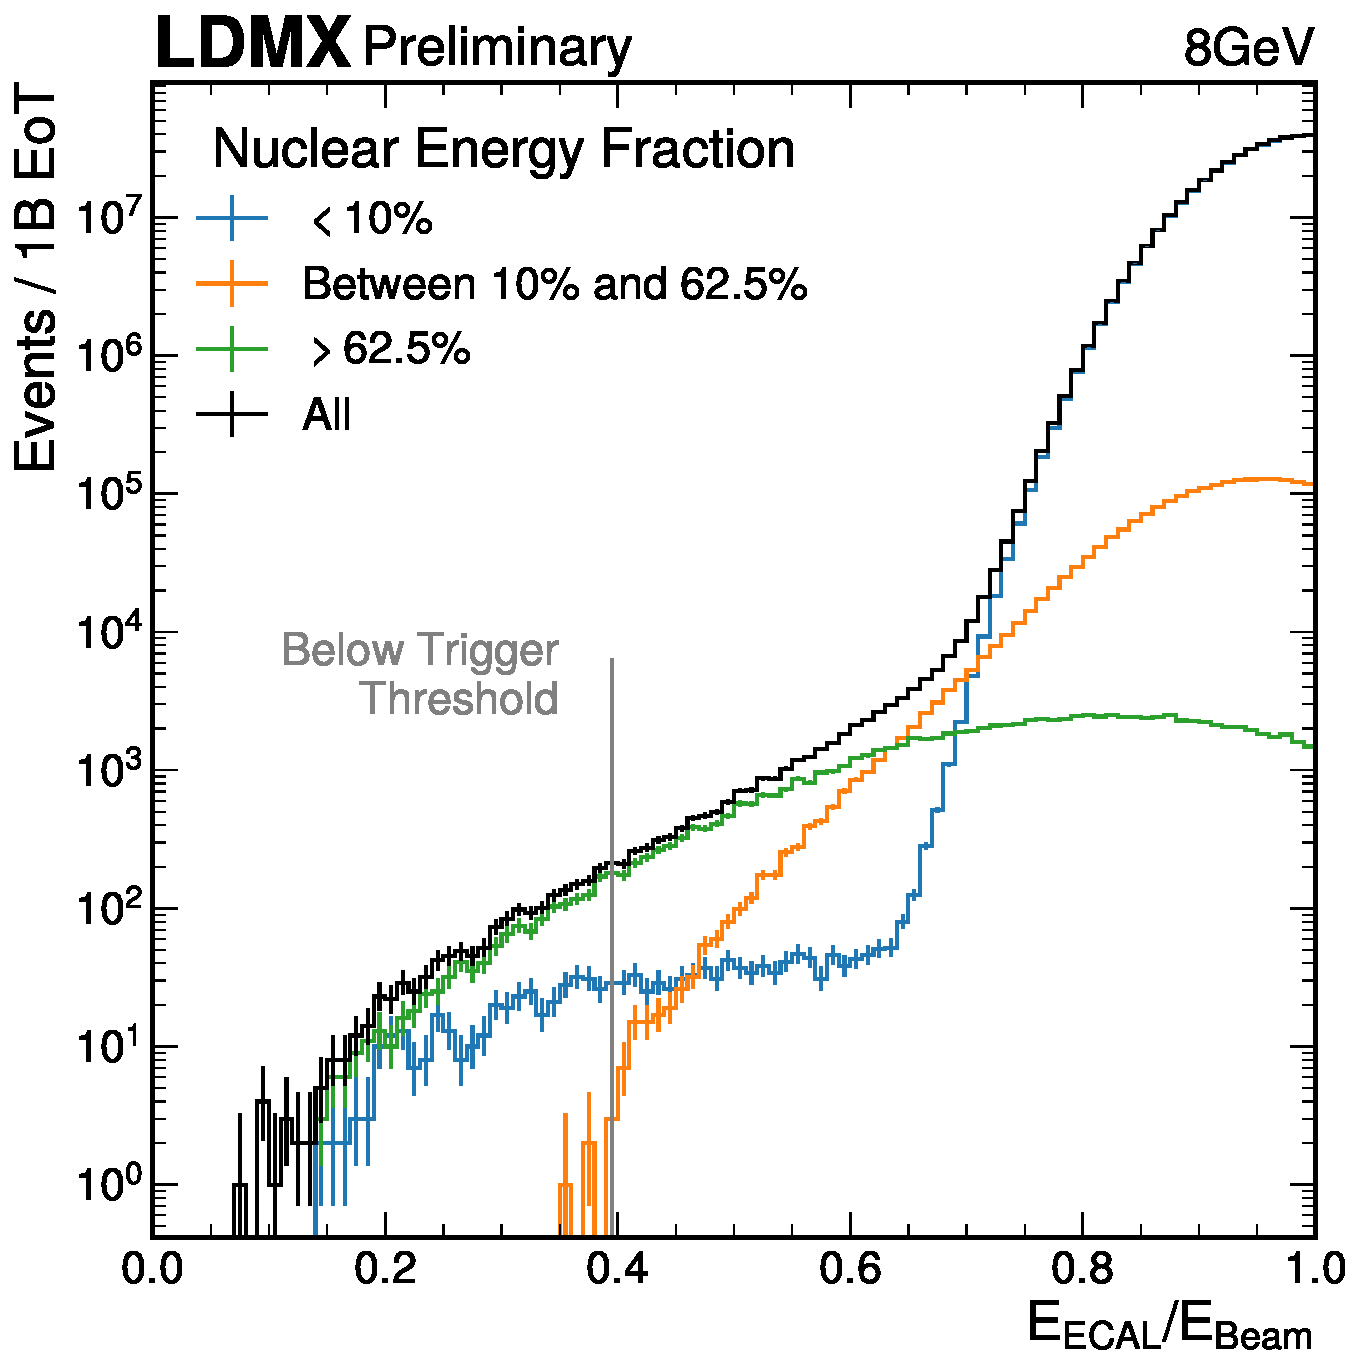
\includegraphics[width=0.9\textwidth]{../figures/ldmx/simulation/8gev-ecal-by-nuc.pdf}
        \caption{\footnotesize Reconstructed energy fraction separated by 
        energy going into nuclear processes.}
      \end{figure}
    \end{column}
    \begin{column}{0.55\textwidth}
      \begin{block}{Simulation Requirement}
        Electron reaches ECal with $> 87.5\%$ of the original beam energy.
      \end{block}

      Standard processes mimicking our signal are similar to thin-target analysis
      \begin{itemize}
        \item ``Nuclear'' processes (electrons and photons interacting with nuclei to produce hadrons)
        \item Muon pair production (via high-energy photon)
      \end{itemize}
    \end{column}
  \end{columns}
\end{frame}

\note[itemize]{
\item The standard processes we need to identify are familiar culprits
  \begin{itemize}
    \item ``Nuclear'' processes
    \item ``Di-Muon'' production via high-energy photons
  \end{itemize}
\item 
}

\subsection{Sensitivity in Early Running}
\begin{frame}{Target Data Volume}
  \begin{columns}
    \begin{column}{0.45\textwidth}
      \begin{figure}
        \centering
        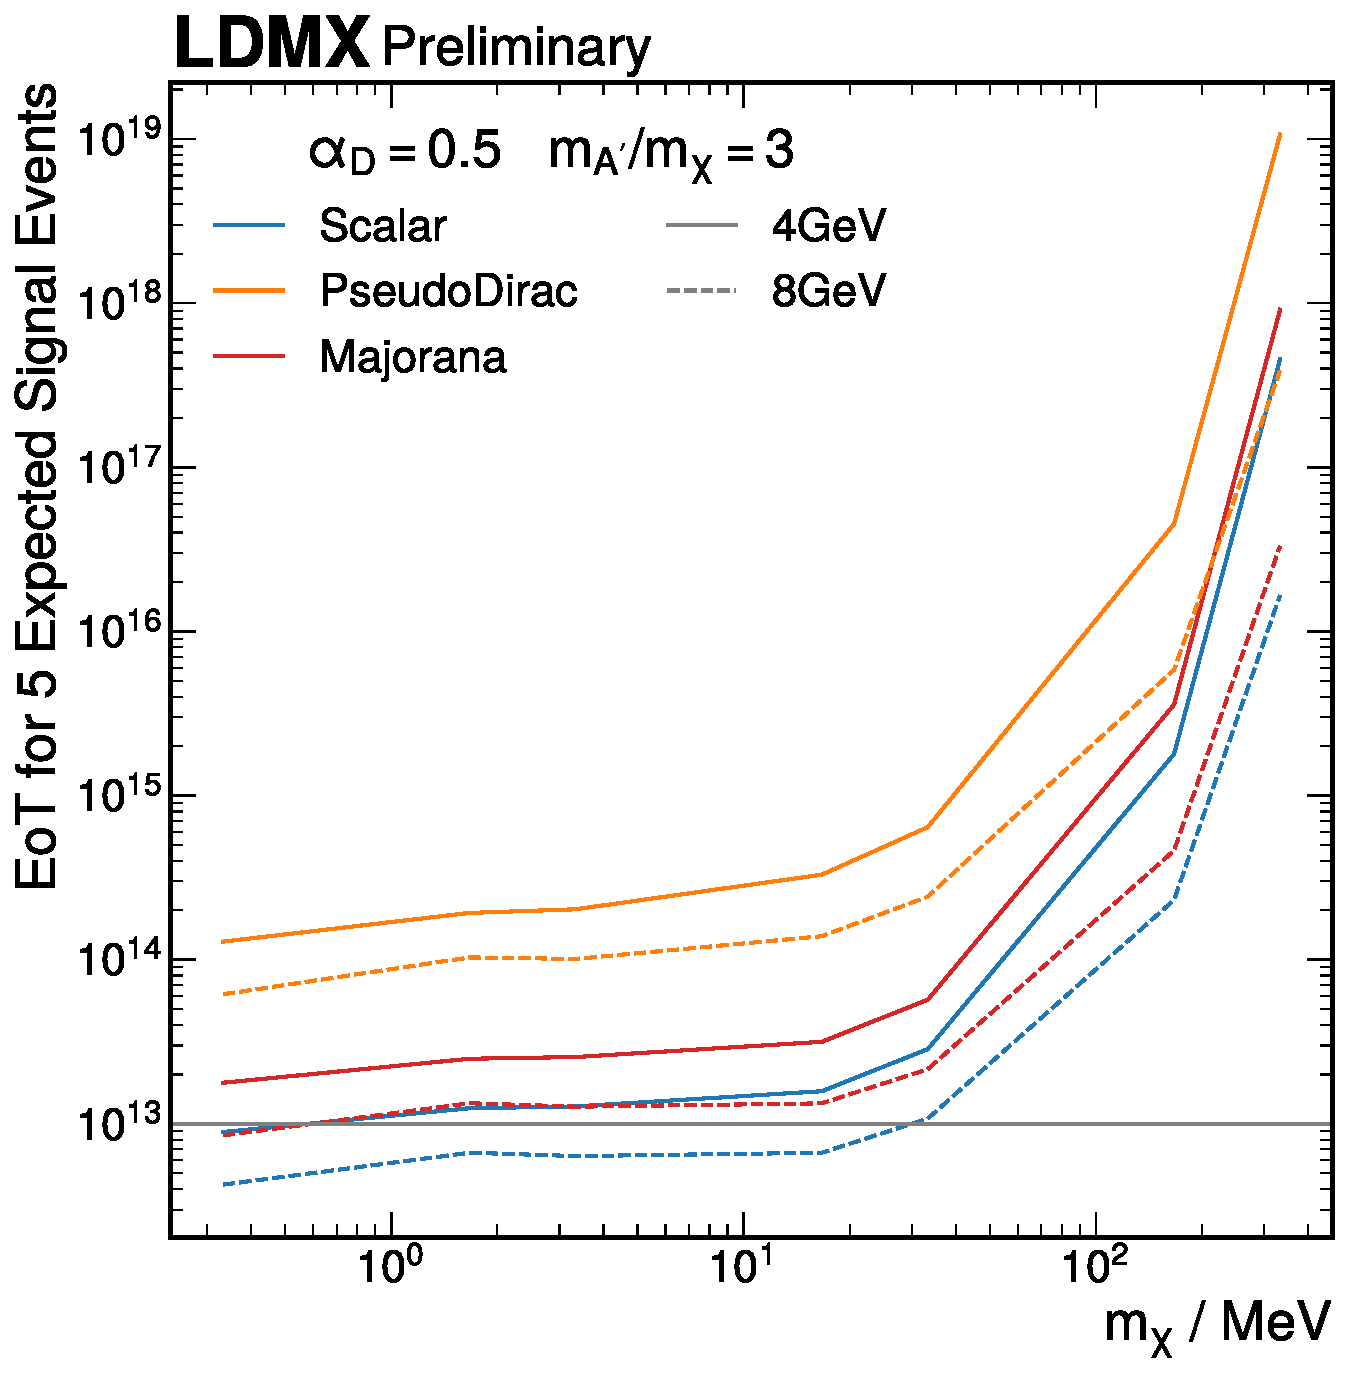
\includegraphics[width=0.9\textwidth]{figs/eot-for-n-signal.pdf}
      \end{figure}
    \end{column}
    \begin{column}{0.55\textwidth}
      \begin{itemize}
        \item Targeting $\sim 5$ expected signal events for a few possible thermal relic models
        \item 
      \end{itemize}
    \end{column}
  \end{columns}
\end{frame}

\begin{frame}{Sensitivity in Early Running}
\end{frame}

\ssection{HPS}

\note[itemize]{
\item HPS takes a different approach towards searching for dark brem
\item Instead of looking for extra events with missing energy/momentum,
  we look for extra events with a specific reconstructed quantities
}

\subsection{Experiment}
\begin{frame}{Experiment}
  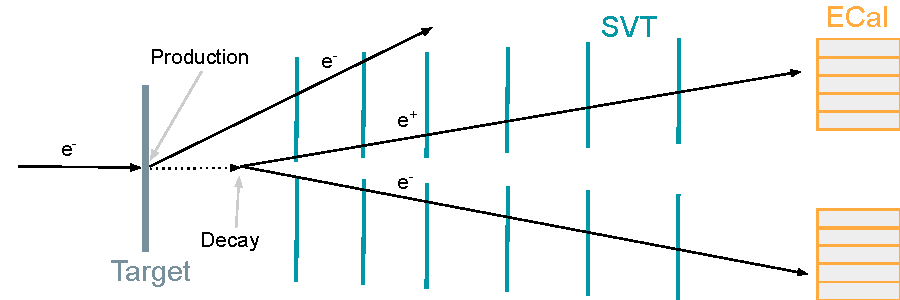
\includegraphics[width=\textwidth]{../figures/hps/experiment/hps-diagram.pdf}
\end{frame}

\note[itemize]{
\item Searching for highly-displaced electron-positron pairs with specific mass
\item High rate of incident electrons to overcome mixing twice
  \begin{itemize}
    \item[$\to$] most pass through thin target without much interaction\
    \item[$\to$] hole in detector to let this high rate of (uninteresting) electrons pass without
  irradiating detector
  \end{itemize}
\item ECal to quickly observe multiple candidate particles and make data collection decision
\item Silicon Vertex Tracker to reconstruct tracks and vertices
\item Benefits
  \begin{itemize}
    \item Physical quantities come with any DM observation
    \item More specific event topology required for standard process to be considered background
  \end{itemize}
\item Downsides
  \begin{itemize}
    \item Need to ``go through'' mixing twice and thus need much higher data volume
    \item Dark sector needs to be ``more defined'' so we can predict
      how it decays back into standard particles
  \end{itemize}
\item Many possible dark sectors yield the correct thermal relic abundance
\item Choose one to focus on for further analysis
}

\subsection{Dark Sector Model}
\begin{frame}{Strongly-Interacting Dark Sector}
  \begin{columns}
    \begin{column}{0.6\textwidth}
      \begin{figure}
        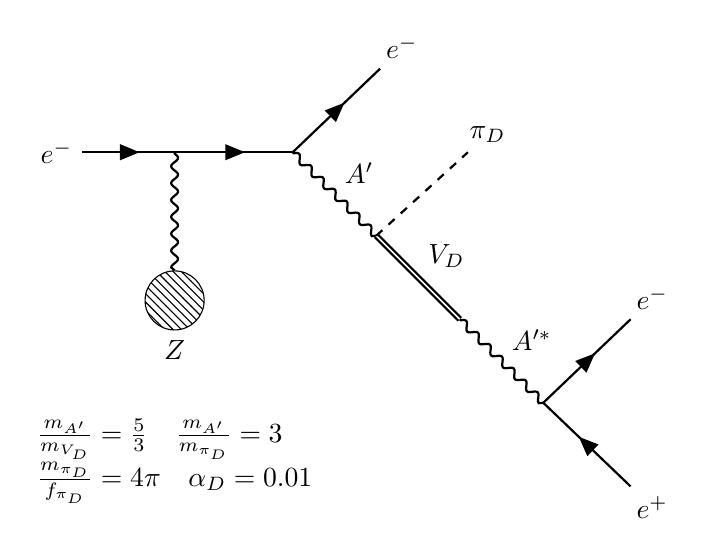
\begin{tikzpicture}
  \begin{feynman}
    \vertex (a) {$e^{-}$};
    \vertex [right= of a](d);
    \vertex [below=of d, blob,label={below:$Z$}] (e) {};
    \vertex [right= of d] (b);
    \vertex [above right= of b] (g) {$e^{-}$};
    \vertex [below right= of b] (aprime_decay);
    \vertex [below right= of aprime_decay] (rhod_decay);
    \vertex [above right= of aprime_decay] (dm) {$\pi_D$};
    \vertex [below right= of rhod_decay] (i);
    \vertex [above right= of i] (j) {$e^{-}$};
    \vertex [below right= of i] (k) {$e^{+}$};
    \diagram*[large] {
    (a) -- [fermion] (d),
    (d) -- [boson] (e),
    (d) -- [fermion] (b),
    (b) -- [fermion] (g),
    (b) -- [boson, edge label={$A'$}] (aprime_decay) -- [double, edge label={$V_D$}] (rhod_decay),
    (aprime_decay) -- [scalar] (dm),
    (rhod_decay) -- [boson, edge label={$A'^*$}] (i),
    (k) -- [fermion] (i) -- [fermion] (j),
    };
  \end{feynman}

  \node [below=of e,align=left] (param)
    {\(\frac{m_{A'}}{m_{V_D}} = \frac{5}{3}\quad\frac{m_{A'}}{m_{\pi_D}} = 3\)\\%
    \(\frac{m_{\pi_D}}{f_{\pi_D}} = 4\pi\quad\alpha_D = 0.01\)};
\end{tikzpicture}

      \end{figure}
    \end{column}
    \begin{column}{0.4\textwidth}
      {\color{UMNMaroon}
      \textbf{S}trongly-\textbf{I}nteracting \\
      \textbf{M}assive \textbf{P}articles
      }
      \begin{itemize}
        \item Dark sector contains ``dark quarks'' -- $\pi_D$ and $V_D$ are mesons like
          standard $\pi$ and $\rho$
        \good Decouples production rate from decay rate
        \bad  Missing energy lost to $\pi_D$ during decay chain
      \end{itemize}
      $$
        m_\mathrm{reco} = m_{V_D} \qquad
        z_\mathrm{reco} \sim e^{-z/(c\tau_{V_D})}
      $$
    \end{column}
  \end{columns}
\end{frame}

\note[itemize]{
\item HPS's 2016 dataset is relatively small meaning a simpler dark sector that has
  the dark photon decaying back to electron-positron pair itself was not reachable
\item SIMPs decouple the production and decay rate allowing real sensitivity for HPS
  within this smaller dataset
}

\subsection{Orthogonal Reconstruction Categories}
\begin{frame}{L1L1 and L1L2}
\end{frame}
\subsection{Cut Optimization Procedure}

\subsection{Subsample Results}

\ssection{Conclusion}

\begin{backup}

\end{backup}

\end{document} 
